\documentclass{article}
\usepackage{amsmath,amsfonts,amsthm,amssymb}
\usepackage{fullpage,fancyhdr}
\usepackage[pdftex]{graphicx}
\usepackage[usenames,dvipsnames]{color}
\usepackage{listings}
\usepackage{courier}
\usepackage{ifthen}
\usepackage{setspace}
\usepackage{lastpage}
\usepackage{extramarks}
\usepackage{chngpage}
\usepackage{soul}
\usepackage{graphicx,float,wrapfig}
\usepackage{epstopdf}
\usepackage{geometry}
\usepackage{pdfcolmk}
\usepackage{hyperref}
\DeclareGraphicsRule{.tif}{png}{.png}{`convert #1 `dirname #1`/`basename #1 .tif`.png}

\definecolor{lightgray}{gray}{0.5}
\definecolor{darkgray}{gray}{0.3}
\definecolor{MyDarkGreen}{rgb}{0.0,0.4,0.0}

\topmargin=-0.45in      %
\evensidemargin=0in     %
\oddsidemargin=0in      %
\textwidth=6.5in        %
\textheight=9.0in       %
\headsep=0.25in         %

\pagestyle{fancyplain}

% For faster processing, load Matlab syntax for listings
\lstloadlanguages{Matlab}%
\lstset{language=Matlab,
        frame=single,
        basicstyle=\ttfamily,
        keywordstyle=[1]\color{Blue}\bf,
        keywordstyle=[2]\color{Purple},
        keywordstyle=[3]\color{Blue}\underbar,
        identifierstyle=,
        commentstyle=\usefont{T1}{pcr}{m}{sl}\color{MyDarkGreen}\small,
        stringstyle=\color{Purple},
        showstringspaces=false,
        tabsize=5,
        % Put standard MATLAB functions not included in the default
        % language here
        morekeywords={xlim,ylim,var,alpha,factorial,poissrnd,normpdf,normcdf},
        % Put MATLAB function parameters here
        morekeywords=[2]{on, off, interp},
        % Put user defined functions here
        morekeywords=[3]{FindESS},
        morecomment=[l][\color{Blue}]{...},
        numbers=left,
        firstnumber=1,
        numberstyle=\tiny\color{Blue},
        stepnumber=5
        }

 
\fancyhf{}
 
\lhead{\fancyplain{}{Michael Carroll}}
\chead{\fancyplain{}{ELEC6410 - DSP}}
\rhead{\fancyplain{}{\today}}
\rfoot{\fancyplain{}{\thepage\ of \pageref{LastPage}}}

\sloppy
\setlength{\parindent}{0pt}

% Alter some LaTeX defaults for better treatment of figures:
% See p.105 of "TeX Unbound" for suggested values.
% See pp. 199-200 of Lamport's "LaTeX" book for details.
%   General parameters, for ALL pages:
\renewcommand{\topfraction}{0.9}	% max fraction of floats at top
\renewcommand{\bottomfraction}{0.8}	% max fraction of floats at bottom
%   Parameters for TEXT pages (not float pages):
\setcounter{topnumber}{2}
\setcounter{bottomnumber}{2}
\setcounter{totalnumber}{4}     % 2 may work better
\setcounter{dbltopnumber}{2}    % for 2-column pages
\renewcommand{\dbltopfraction}{0.9}	% fit big float above 2-col. text
\renewcommand{\textfraction}{0.07}	% allow minimal text w. figs
%   Parameters for FLOAT pages (not text pages):
\renewcommand{\floatpagefraction}{0.7}	% require fuller float pages
% N.B.: floatpagefraction MUST be less than topfraction !!
\renewcommand{\dblfloatpagefraction}{0.7}	% require fuller float pages
% remember to use [htp] or [htpb] for placement

\linespread{1.3}

\title{ELEC6410 Project 6\\
 {\large \begin{par}
Answers to Digital Signal Processing Project \#6
\end{par}
}}
\author{Michael J. Carroll}

\begin{document}
\maketitle
           
\section*{Exercise 1}
\begin{par}
For exercise 1, I evaluated four of  built-in filter functions.  The goal was to design a 5th-order lowpass IIR filter of each of the different types.  The passband cutoff was $0.15\pi$, the passband ripple was to be 0.5 dB, and the maximum stop band ripple was to be 30 dB.  For each filter, I created a phase-magnitude plot, a z-plane plot, and an impulse response function.\\
\\
In Figures 1, 2, and 3 are the detailed plots for the output of the MATLAB \texttt{butter} command.  The magnitude plot reflects the Zero-Pole plot, as the plot is smooth and continuous, due to the fact that there are no poles or zeros on the unit circle until high frequencies are reached.  Once the higher frequencies are reached, the magnitude response quickly drops, as to be expected.\\
\\
Figures 4, 5, and 6 are the detailed plots for the output of the MATLAB \texttt{cheby1} command.  The magnitude plot is almost identical to that of the Butterworth Filter.  The design that I used minimized stopband ripple, so it stands to reason that the plot will be remarkably similar to the Butterworth filter, as is the Zero-Pole plot in Figure 5.\\
\end{par}
\begin{par}
Figures 7, 8, and 9 are the detailed plots for the \texttt{cheby2} command.  The \texttt{cheby2} command also generates a Chebyshev type filter, but with more stopband ripple, as is visible in Figure 7.  The zeros present on the unit circle in the Zero-Pole plot of the Chebyshev type II filter in Figure 8 cause the magnitude response to quickly drop at two points, which is present in the magnitude response plot in Figure 7.\\
\\
Figures 10, 11, and 12 are the plots for the \texttt{ellip} command.  The elliptical filter magnitude response (Figure 10) and Zero-Pole plot (Figure 11) are similar to the Chebyshev type II filter in the previous step, but with a much tighter transition band, which is a characteristic of the elliptic filter.\\
\\
The performance of the four filters can be evaluated based on "flatness", phase-response, and transition band width.  The use of the filter will drive the selection of the IIR filter for the most part.  To a large degree, the "smoothness" of the pass-band and stop-band can drive the selection towards a Chebyshev type I or II filter, depending on which band is required.  A sharper transition band would yield itself to an elliptic filter design.  If phase response is a critical component of the design, then the Butterworth filter would prove to be the best design.\\
\\
As far as we have studied, the impulse responses of all of the filters appear to be lowpass.  They have large, sweeping curves that look like some form of the sinc function.
\end{par}

\begin{figure}[htb]
\begin{minipage}[b]{0.5\linewidth}
\centering
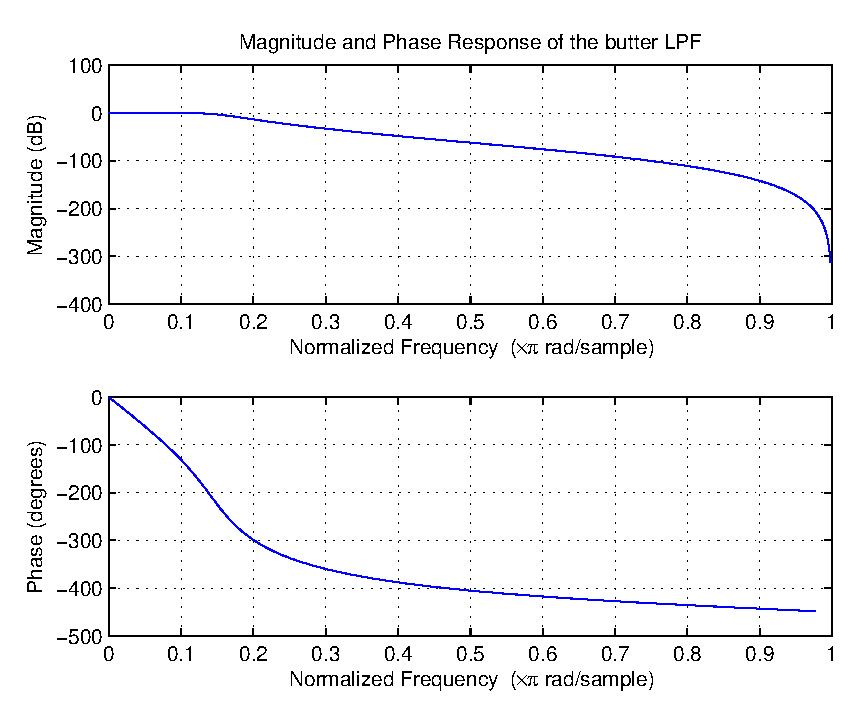
\includegraphics[width=3in]{project6_01.eps}
\caption{Magnitude-Phase of  Butterworth LPF}
\label{fig:figure1}
\end{minipage}
\hspace{0.5cm}
\begin{minipage}[b]{0.5\linewidth}
\centering
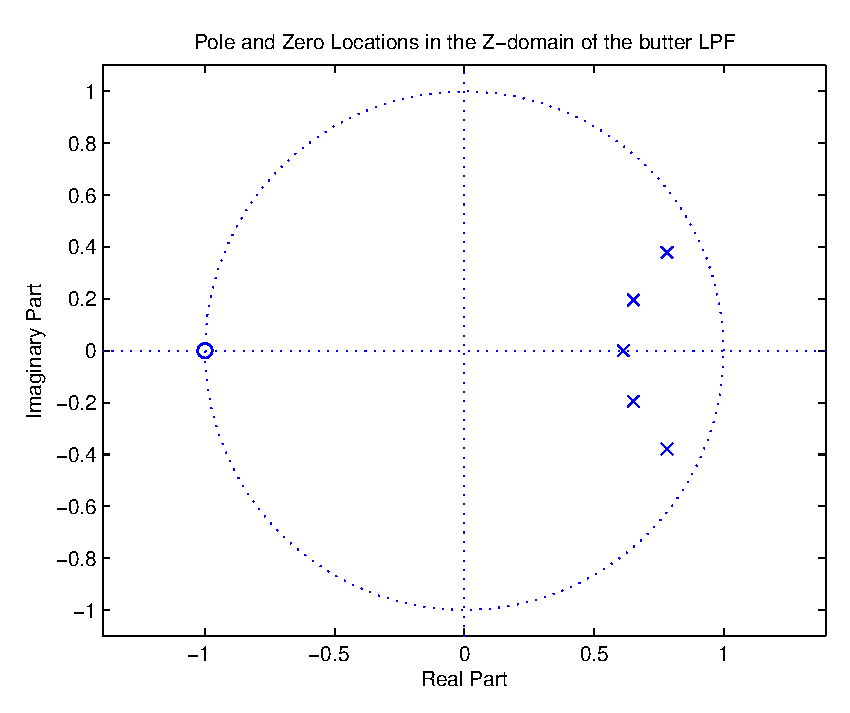
\includegraphics[width=3in]{project6_02.eps}
\caption{Pole-Zero Locations of  Butterworth LPF}
\label{fig:figure2}
\end{minipage}
\end{figure}

\begin{figure}[htb]
\begin{minipage}[b]{0.5\linewidth}
\centering
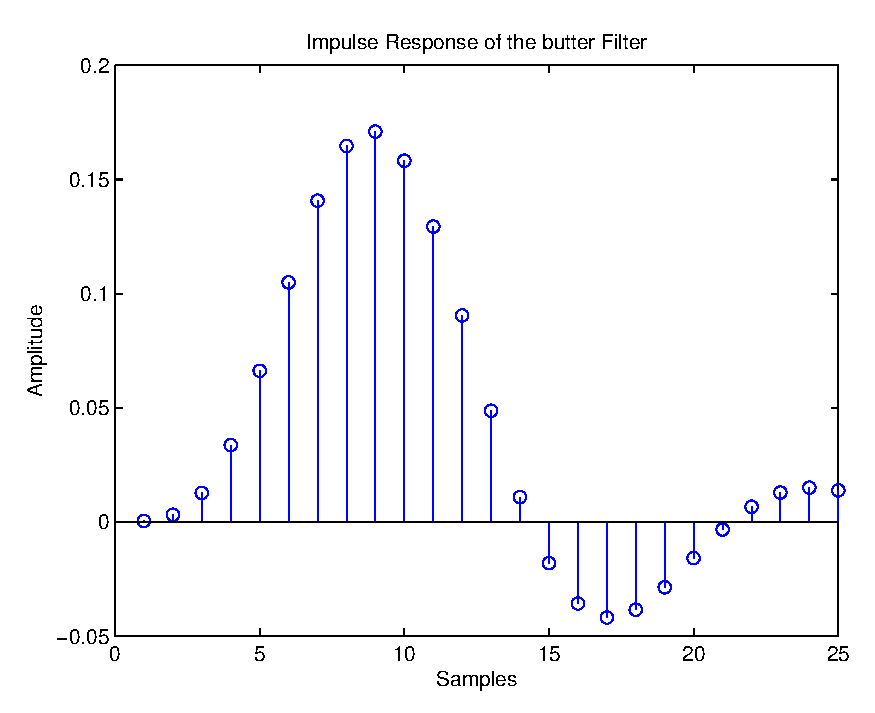
\includegraphics[width=3in]{project6_03.eps}
\caption{Impulse Response of  Butterworth LPF}
\label{fig:figure3}
\end{minipage}
\hspace{0.5cm}
\begin{minipage}[b]{0.5\linewidth}
\centering
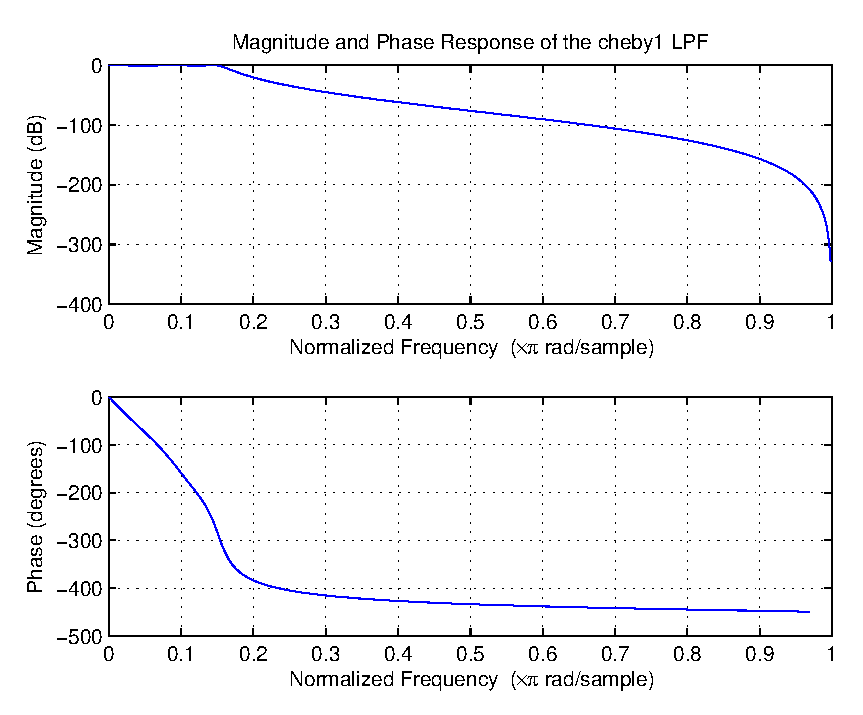
\includegraphics[width=3in]{project6_04.eps}
\caption{Magnitude-Phase of  Chebyshev I LPF }
\label{fig:figure4}
\end{minipage}
\end{figure}

\begin{figure}[htb]
\begin{minipage}[b]{0.5\linewidth}
\centering
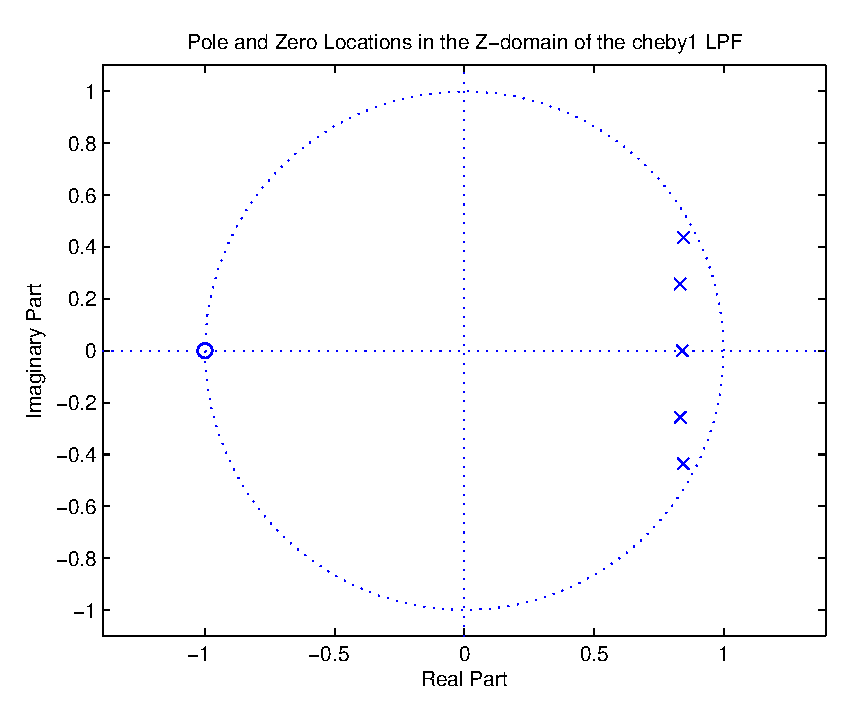
\includegraphics[width=3in]{project6_05.eps}
\caption{Pole-Zero Locations of  Chebyshev I LPF}
\label{fig:figure5}
\end{minipage}
\hspace{0.5cm}
\begin{minipage}[b]{0.5\linewidth}
\centering
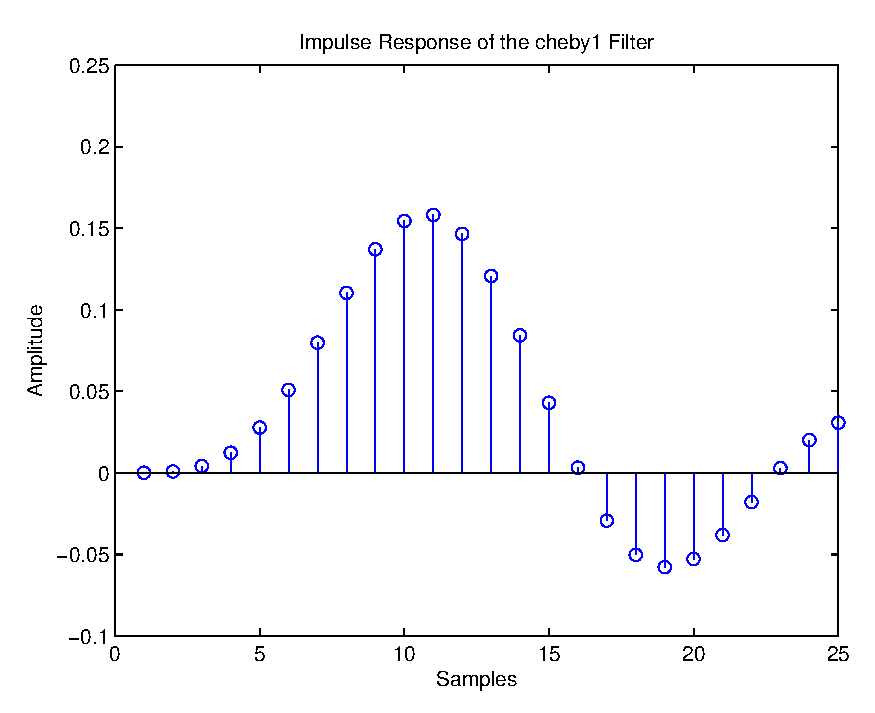
\includegraphics[width=3in]{project6_06.eps}
\caption{Impulse Response of  Chebyshev I LPF}
\label{fig:figure6}
\end{minipage}
\end{figure}

\begin{figure}[ht]
\begin{minipage}[b]{0.5\linewidth}
\centering
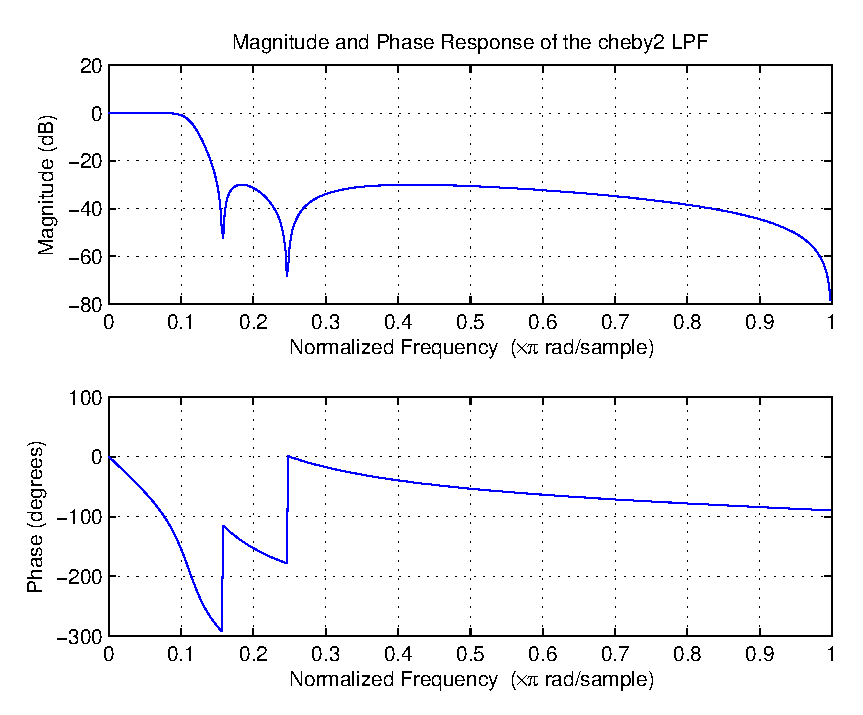
\includegraphics[width=3in]{project6_07.eps}
\caption{Magnitude-Phase of  Chebyshev II LPF}
\label{fig:figure7}
\end{minipage}
\hspace{0.5cm}
\begin{minipage}[b]{0.5\linewidth}
\centering
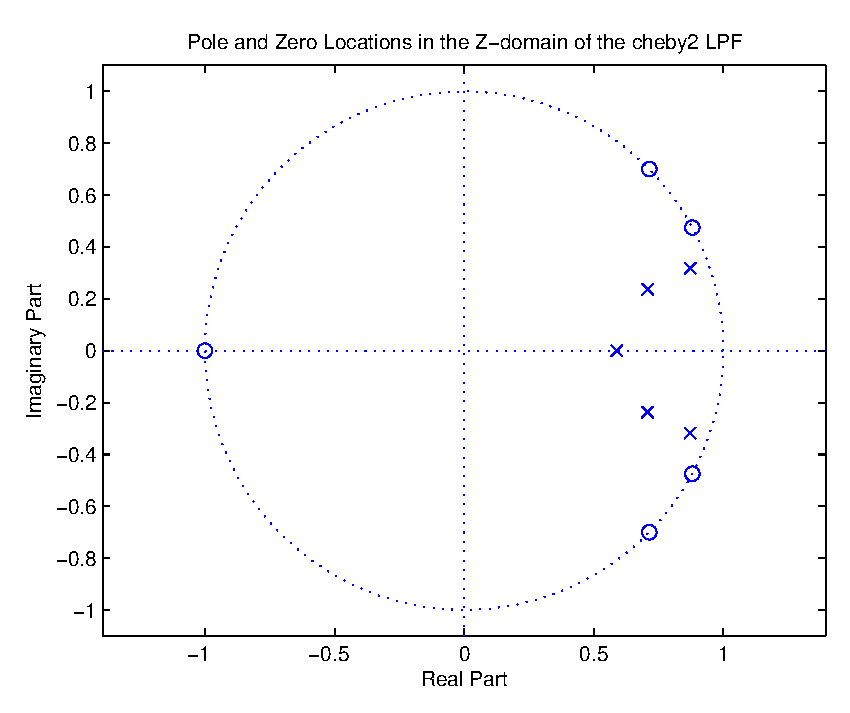
\includegraphics[width=3in]{project6_08.eps}
\caption{Pole-Zero Locations of  Chebyshev II LPF}
\label{fig:figure8}
\end{minipage}
\end{figure}

\begin{figure}[ht]
\begin{minipage}[b]{0.5\linewidth}
\centering
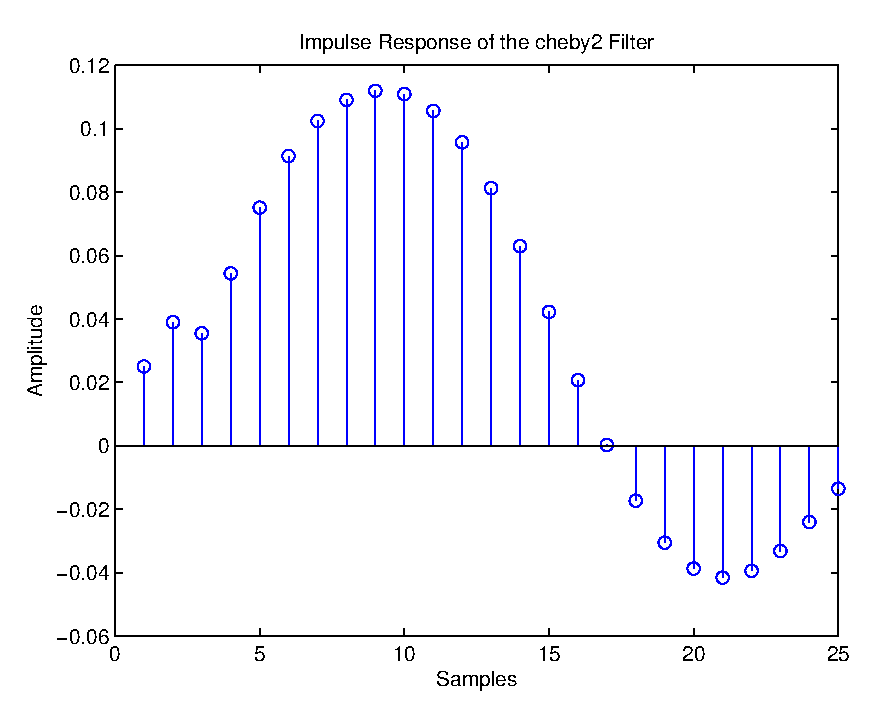
\includegraphics[width=3in]{project6_09.eps}
\caption{Impulse Response of  Chebyshev II LPF}
\label{fig:figure9}
\end{minipage}
\hspace{0.5cm}
\begin{minipage}[b]{0.5\linewidth}
\centering
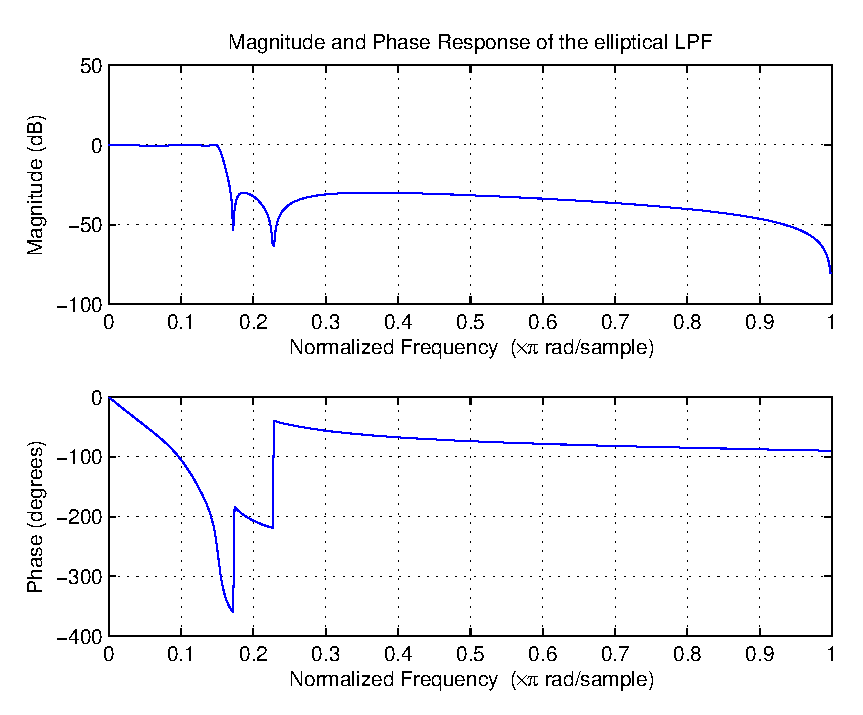
\includegraphics[width=3in]{project6_10.eps}
\caption{Magnitude-Phase of  Elliptical LPF}
\label{fig:figure10}
\end{minipage}
\end{figure}

\begin{figure}[ht]
\begin{minipage}[b]{0.5\linewidth}
\centering
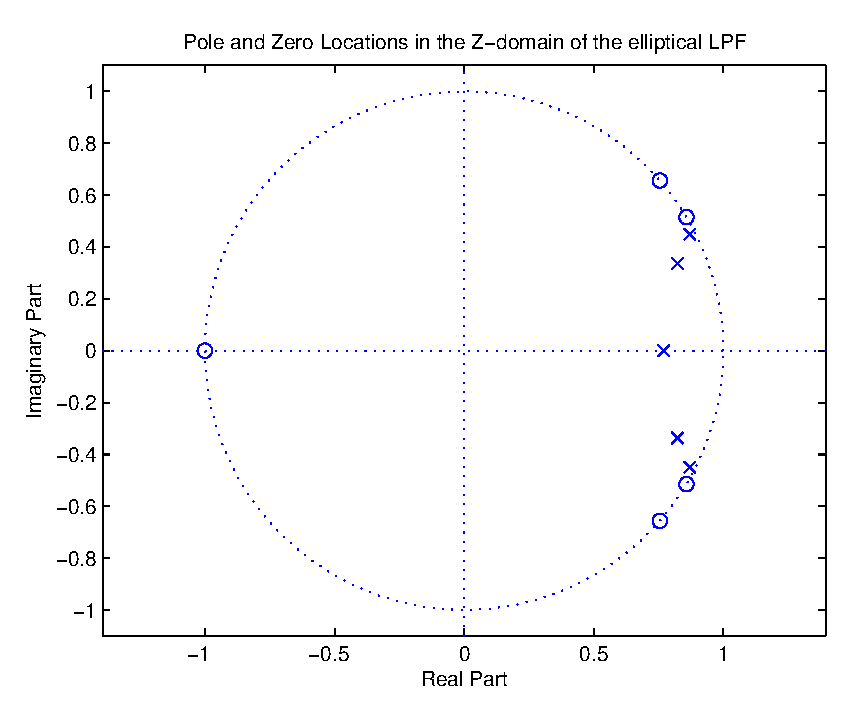
\includegraphics[width=3in]{project6_11.eps}
\caption{Pole-Zero Locations of Elliptical LPF}
\label{fig:figure11}
\end{minipage}
\hspace{0.5cm}
\begin{minipage}[b]{0.5\linewidth}
\centering
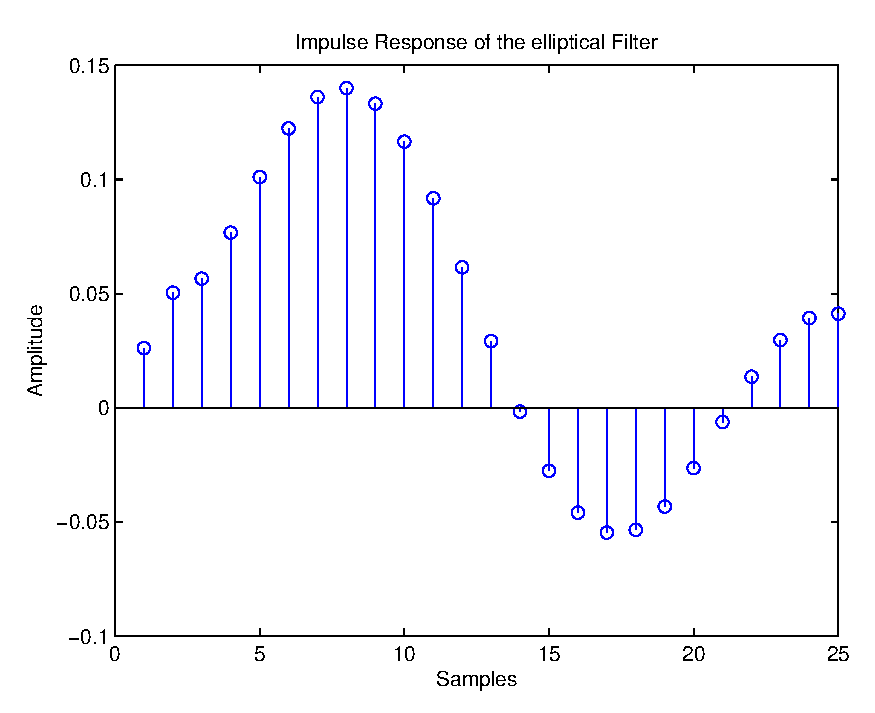
\includegraphics[width=3in]{project6_12.eps}
\caption{Impulse Response of  Elliptical LPF}
\label{fig:figure12}
\end{minipage}
\end{figure}

\newpage

\section*{Exercise 2}
\begin{par}
For the second part of the lab, I compared the order of the different types of filters with the same design specifications.  I accomplished this using the \texttt{buttord, cheb1ord, cheb2ord,} and \texttt{ellipord} commands.
\end{par}
\begin{verbatim}
Butterworth Order: 3
Chebyshev I Order: 3
Chebyshev II Order: 3
Elliptical Order: 2
\end{verbatim}

\begin{par}
The Elliptical filter has an order less than that of other filters.  The reason for this is the sharp transition band of the elliptical filter.  This guarantees that the filter can meet the design specification of the pass and stop band positions with a lower order than the other filters.
\end{par}

\section*{Exercise 3}
\begin{par}
In Exercise 3, I analyzed the frequency spectrum of the provided "doorbell.au" file.  I accomplished this using MATLAB's built in \texttt{fft} command.  The output of the command is included in Figure 13, where the principal frequencies are 712 Hz (for the higher pitch) and 567 Hz (for the lower pitch).  This gives the frequencies of the pass and stop bands for the lowpass filters. \\
\\
Using the frequencies and the upper and lower attenuation levels in the problem description, I designed the four filters that I have been experimenting with.  Once again, the Elliptical filter features the lowest order of all of the filters.  This is because the narrow transition band once again allows me to hit the design requirements with a lower order.\\
\\
After listening to the original, I listened to each of the filter's outputs.  Each filter has a bit different "feel" to the output sound, but all of the filters attenuate the high frequency sound.
\end{par}

%\begin{table}[tbph]
%\begin{center}
%\begin{tabular}{| l | r | r |}
%\hline
%Filter Type & Low Frequency Attenuation & High Frequency Attenuation \\
%\hline
%Butterworth & 2.63 dB & 17.25 dB \\
%Chebyshev I & 3.51 dB & 21.85 dB \\
%Chebyshev II & 0.15 dB & 16.27 dB \\
%Elliptical & 3.56 dB & 19.7 dB \\
%\hline
%\end{tabular}
%\end{center}
%\end{table}

\begin{lstlisting}
Wp = 567* 2/8000; Ws = 712 * 2/8000;
Rp = 3;  Rs = 15;

[Nb,Wnb] = buttord(Wp, Ws, Rp, Rs);
[Bb,Ab] = butter(Nb,Wnb,'low');
yb = filter(Bb,Ab,audio);
[Nc1,Wnc1] = cheb1ord(Wp, Ws, Rp, Rs);
[Bc1,Ac1] = cheby1(Nc1,Rp,Wnc1,'low');
yc1 = filter(Bc1,Ac1,audio);
[Nc2,Wnc2] = cheb2ord(Wp, Ws, Rp, Rs);
[Bc2,Ac2] = cheby2(Nc2,Rp, Wnc2,'low');
yc2 = filter(Bc2,Ac2,audio);
[Ne,Wne] = ellipord(Wp, Ws, Rp, Rs);
[Be,Ae] = ellip(Ne,Rp,Rs,Wne,'low');
ye = filter(Be,Ae,audio);
\end{lstlisting}

\begin{verbatim}
Butterworth Order: 8
Chebyshev I Order: 4
Chebyshev II Order: 4
Elliptical Order: 3
\end{verbatim}

\begin{figure}[htbp]
\centering
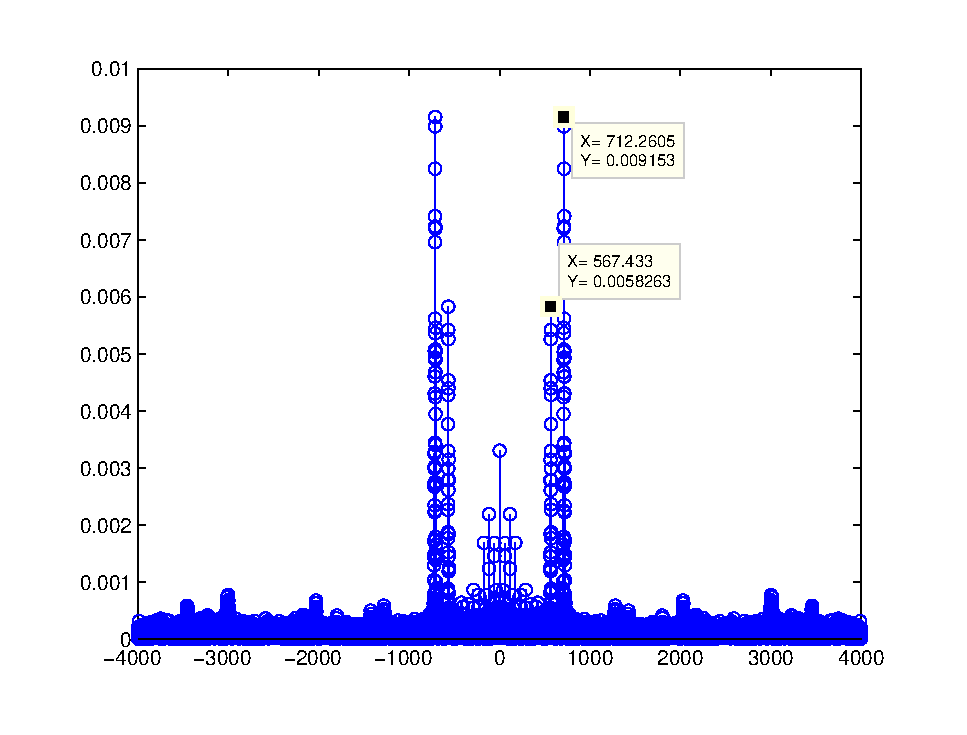
\includegraphics[width=4in]{project6_part3.eps}
\caption{Frequency Spectrum of doorbell.au}
\label{fig:figure13}
\end{figure}


\end{document}

